\providecommand{\atd}{..}
\documentclass[../main.tex]{subfiles}

\begin{document}
    \chapter{Behavior Line}\label{ch:behavior-line}
    \section{Description}\label{sec:description2}
    In the behavior line we wanted to specify the typical interaction that the user has with the system. Perhaps our subject will be the primary persona previously identified. We decided to focus on the interaction rather than the pre-sale phase, because we thought that the pre-sale would have been heavily influenced by the fact that the system is for exclusive use of authorities: this would imply a lot of bureaucratic steps and deals that don’t depend only from us and from our possible marketing choices.
    In a possible typical interaction, we decided to apply the context of the beginning of a pandemic situation, like the Covid-19 one. Beside from that, as stated in some notes attached to the Behavior Line, the system’s functionalities are not limited to a pandemic situation.
    We identified a path starting from the powering on of the PC used to access the system and going through the different functionalities available and accessible in a likely task routine. The first main step (and touch point with the system) is the home page, then we identified the visualization of the results of a search, the page that allows to set up scheduled analysis and finally the feature that allow the creation of dashboard in order to create reports of what has been observed. We could have identified another main step: the search page, which we decided to omit from the template since is something more technical and somehow incorporated in the results page (where we can perform more detailed search starting from the results of a previous one).

    \section{Behavior Line Template}\label{sec:behavior-line-template}
    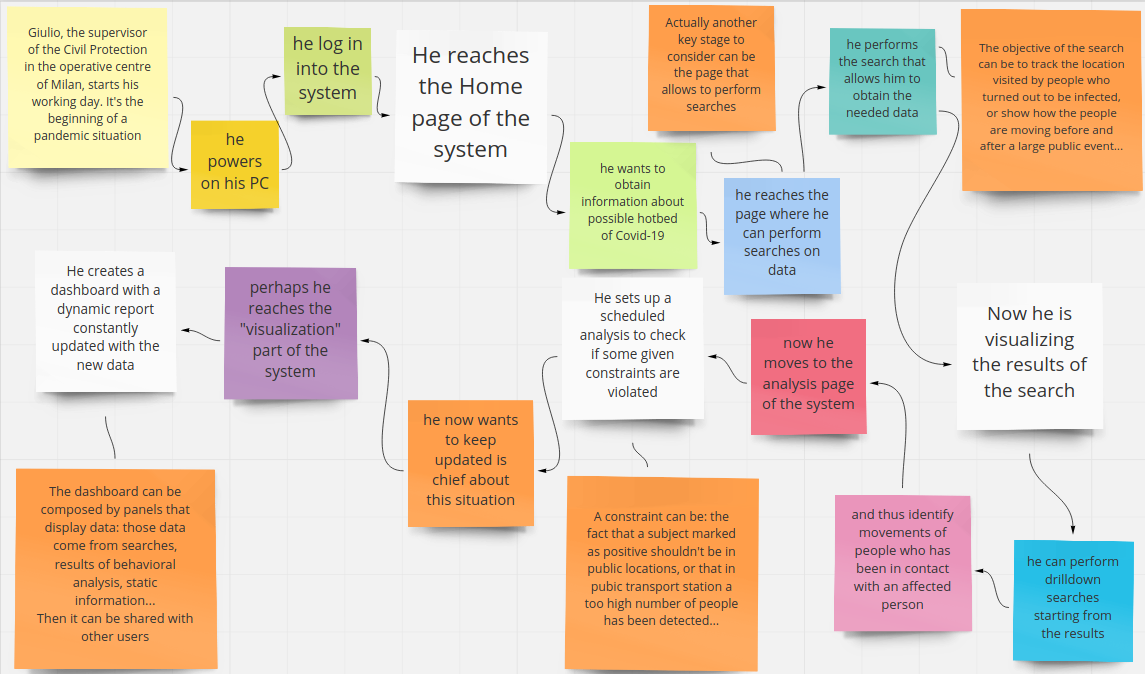
\includegraphics[scale = 0.4]{assets/behavior_line.png}
    \chapter{Customer Journey}\label{ch:customer-journey}
    \section{Description}\label{sec:description}
    In this template we are able to specify the main step identified in the Behavior Line. For each of them the touch points are listed: the most important are highlighted in green. In the case of the Home Page, we considered the navigation menu as very important, since from here the user should be able to reach every section of the system without too much effort. A metric to measure the effectiveness of the navigation menu is the number of click to reach a certain area of the system. We gave less importance to a possible informative section located in the home page: this section can display general information like the state of the system, the user logged in, the software version…
    About the page that allows to visualize the results we considered the map visualization as a key point: since we are tracking people behavior while moving around the city, a proper visualization through a map is probably the most important. Then also the tools that allow to refine the search must be clear and user friendly. One possible improvement that can be implemented is a new visualization paradigm: after users feedback it will be possible to figure out new kind of useful visualization.
    In the section that allow the creation of behavioural scheduled analysis, the most important touch point identified is the insertion of the constraint that the analysis will have to check: the challenge is defining a standard way to formally define different constraint. Other settings (like how many times the scheduled analysis have to run, on which timespan ecc…) are considered as less complicated.
    Finally, in the dashboard creation, a useful tool which the user will use is a “drag and drop” that will allow the composition of a dashboard with standard elements. Then the user will be allowed (if he wants, it’s optional) to customize these elements. What we considered also as very important is the permission setting of the dashboard: when creating a dashboard, it must be clear who the user is sharing it with. Here a possible future implementation is the insertion of elements developed by third-parties in the dashboard visualization: in this way it’s possible to improve the effectiveness of the dashboard in visualizing data and also it will be possible to introduce active behavior right into the dashboard.

    \section{Customer Journey Template}\label{sec:customer-journey-template}
    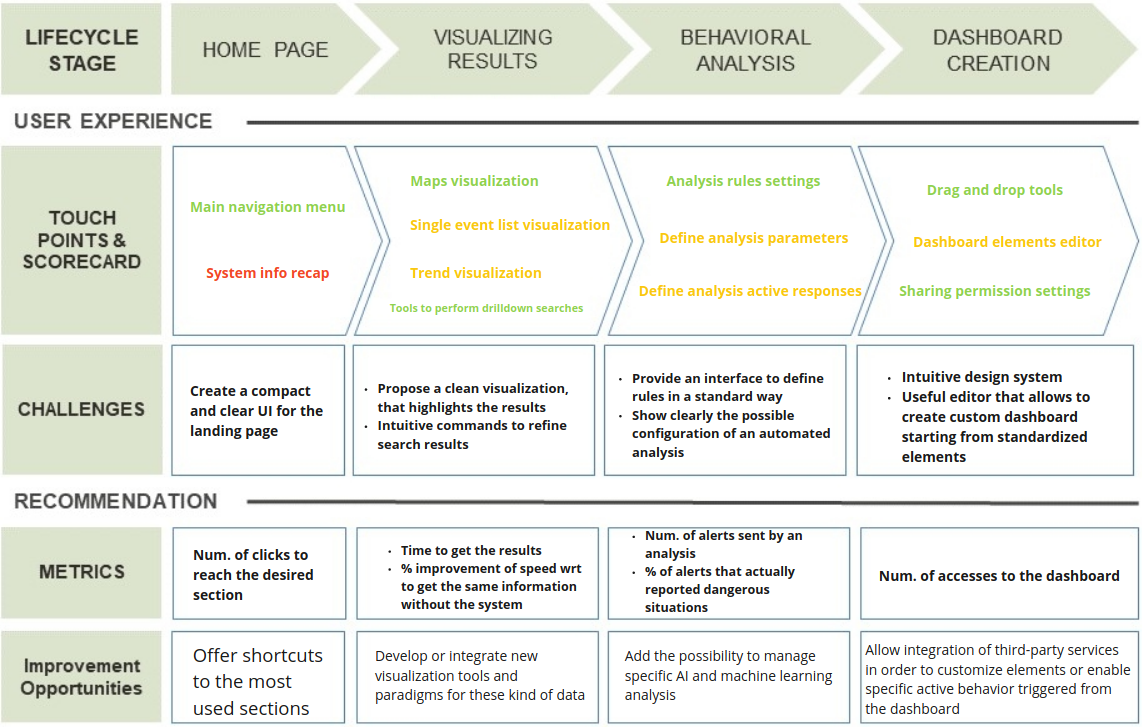
\includegraphics[scale = 0.4]{assets/customer_journey.png}
\end{document}